\chapter{Analyse}

\section{Übersicht}

\subsection{Gesamtprogramm}

Messungen des Gesamtprogramms (Datentransfers, alle Stufen)

\subsection{Teilstufen}

grobe Messungen der Teilstufen (Wichtung, Filterung, Rückprojektion)

Ergebnis: Rückprojektion braucht am längsten

\section{Eigenschaften des Rückprojektionskernels}

\subsection{Ressourcenverbrauch}

\subsection{Auslastung}

\subsection{Wartezeiten}

Eines der drei Optimierungsziele, die in Abschnitt~\ref{ssec:opti_ueber} genannt wurden, ist die Verkürzung der Wartezeit
zwischen dem Ende einer Rückprojektion und dem Beginn der nachfolgenden Rückprojektion. Zu diesem Zweck wird die
Rückprojektion in einem eigenen Thread und \gls{cuda}-Stream ausgeführt, sodass die vorherigen Operationen (Laden,
Wichten, Filtern) parallel zur Rückprojektion ausgeführt werden können. Der Rückprojektionsthread entnimmt die nächste
Projektion vom Stapel der noch ausstehenden Projektionen, wandelt diese in eine \gls{cuda}-Textur um und startet dann
den Rückprojektions-\gls{kernel}. Wie Abbildung~\ref{fig:kernel_wait} zeigt, ist es gelungen, die Zeit zwischen zwei
Rückprojektionen, die durch die langen, grün-blauen Balken dargestellt werden, auf 3 Millisekunden zu beschränken. Bei
einem üblichen Datensatz von 1440 Projektionen ergibt sich also eine Gesamtwartezeit von 4,32 Sekunden.

Abbildung~\ref{fig:kernel_wait} zeigt allerdings auch, dass diese Wartezeit noch nicht ideal ist. Das Ziel, die Wichtung
und die Filterung, die durch die kleineren, bunten Balken repräsentiert werden, parallel zur Rückprojektion
durchzuführen, konnte nicht erreicht werden. Der Grund dafür ist vermutlich die Anzahl der Threads, die vom
Rückprojektions-\gls{kernel} gestartet werden. Bei einem Volumen mit 1070 x 1070 x 1033 \gls{voxel}n, denen jeweils ein
Thread zugeordnet wird, werden 1.182.681.700 Threads benötigt. Die hier verwendete Grafikkarte, die
GeForce{\textregistered} GTX 1080, verfügt über 20 \gls{sm}s, von denen jeder bis zu 2.048 Threads gleichzeitig
ausführen kann und kann somit bis zu 40.960 Threads gleichzeitig verwalten. Die \gls{gpu} ist daher gezwungen, der
Rückprojektion alle verfügbaren Threads zuzuweisen, was zur Folge hat, dass keine weiteren \gls{kernel} ausgeführt
werden können.

Der schwerwiegendere Einfluss geht jedoch von der Umwandlung der Projektionen in \gls{cuda}-Texturen bzw. der Erzeugung
letzterer aus, wie Abbildung~\ref{fig:kernel_tex} zeigt (orange markiert). Mit etwa 1,7 Millisekunden (siehe
Abbildung~\ref{fig:kernel_tex_prop}) nimmt dieser Prozess mehr als die Hälfte der Wartezeit ein.

Grundsätzlich lässt sich feststellen, dass die Wartezeit zwischen zwei Rückprojektionen, die über die gesamte Laufzeit
etwas mehr als 4 Sekunden einnimmt, einen akzeptablen Wert erreicht hat, der dem alltäglichen Gebrauch nicht im Wege
steht. Auch wenn an dieser Stelle noch Optimierungspotential vorhanden ist, brächte selbst eine vollständige
Eliminierung der Wartezeit keinen besonders hervorzuhebenden Mehrwert.

\begin{figure}
    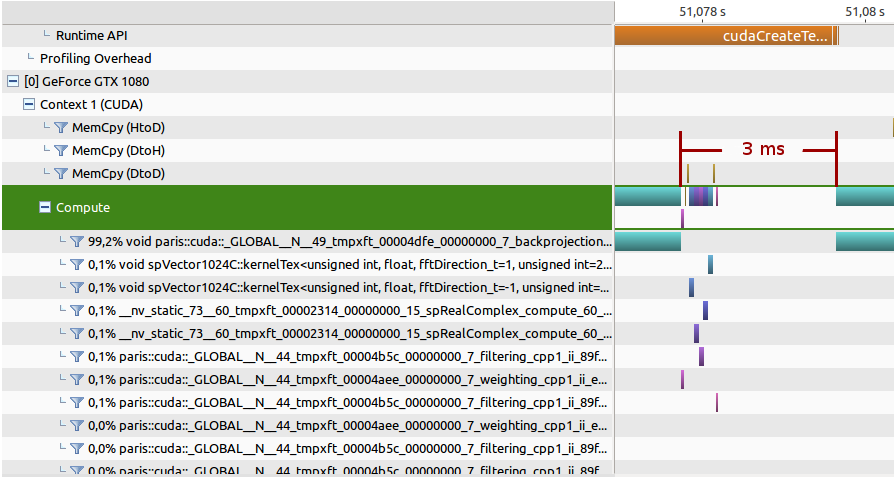
\includegraphics[width=\linewidth]{img/timeline_compute2}
    \caption{Zeit zwischen zwei Rückprojektionen}
    \label{fig:kernel_wait}
\end{figure}

\begin{figure}
    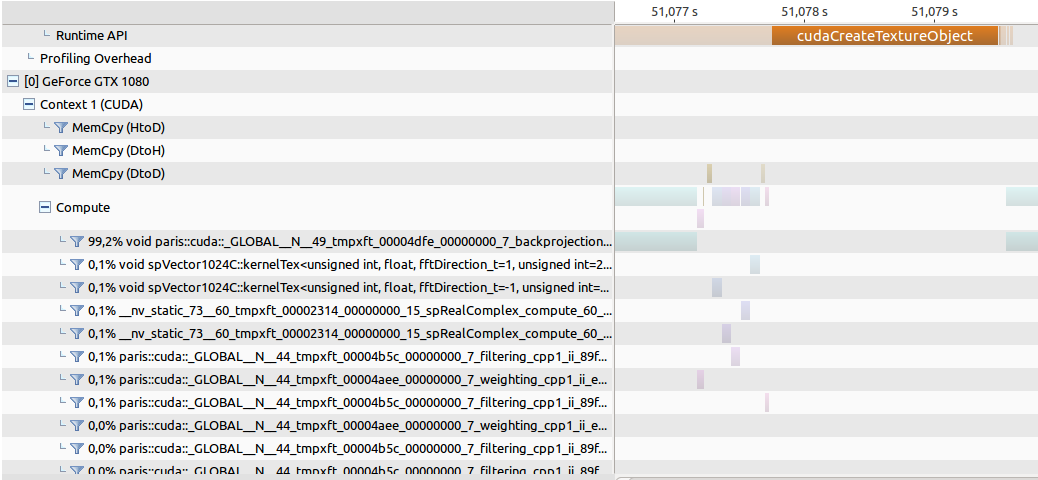
\includegraphics[width=\linewidth]{img/timeline_texture2}
    \caption{Die Texturerzeugung macht den größten Teil der Wartezeit aus}
    \label{fig:kernel_tex}
\end{figure}

\begin{figure}
    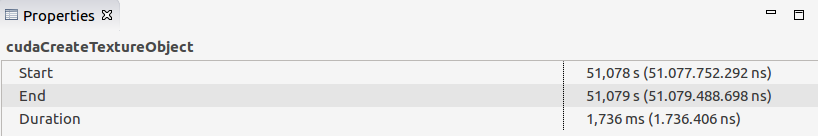
\includegraphics[width=\linewidth]{img/timeline_texture_properties}
    \caption{Ausführungszeit der \gls{cuda}-Texturerzeugung}
    \label{fig:kernel_tex_prop}
\end{figure}

\subsection{Laufzeit}

\subsection{Einsatz mehrerer \gls{gpu}s}

\begin{figure}
    \centering
    \begin{tikzpicture}
        \begin{axis}[width=\textwidth,
                     xlabel={Volumengröße},
                     symbolic x coords={133 x 133 x 129,267 x 267 x 258,535 x 535 x 516, 1070 x 1070 x 1033},
                     xtick=data,
            %                     x tick label style={rotate=45,anchor=east},
                     ylabel={Laufzeit [s]}]

             \addplot table[x=Volumengroesse,y=GTX1080,col sep=comma] {data/mehreregpus.csv};
             \addplot table[x=Volumengroesse,y=K20c,col sep=comma] {data/mehreregpus.csv};
             \addplot table[x=Volumengroesse,y=GTX1080K20c,col sep=comma] {data/mehreregpus.csv};
             \legend{GTX 1080,Tesla K20c,GTX+Tesla};
        \end{axis}
    \end{tikzpicture}
    \caption{Laufzeit mit mehreren \gls{gpu}s}
    \label{fig:laufzeit_gpus}
\end{figure}

\section{Vergleich mit der Literatur}
